%iffalse
\let\negmedspace\undefined
\let\negthickspace\undefined
\documentclass[journal,12pt,onecolumn]{IEEEtran}
\usepackage{cite}
\usepackage{amsmath,amssymb,amsfonts,amsthm}
\usepackage{algorithmic}
\usepackage{graphicx}
\usepackage{textcomp}
\usepackage{xcolor}
\usepackage{txfonts}
\usepackage{listings}
\usepackage{enumitem}
\usepackage{mathtools}
\usepackage{gensymb}
\usepackage{comment}
\usepackage[breaklinks=true]{hyperref}
\usepackage{tkz-euclide} 
\usepackage{listings}
\usepackage{gvv}                                        
% \usepackage{gvv}  
\usepackage[latin1] {inputenc}
\usepackage{xparse}
\usepackage{color}                                            
\usepackage{array}                                            
\usepackage{longtable}                                       
\usepackage{calc}                                             
\usepackage{multirow}
\usepackage{multicol}
\usepackage{hhline}                                           
\usepackage{ifthen}                                           
\usepackage{lscape}
\usepackage{tabularx}
\usepackage{array}
\usepackage{float}
\newtheorem{theorem}{Theorem}[section]
\newtheorem{problem}{Problem}
\newtheorem{proposition}{Proposition}[section]
\newtheorem{lemma}{Lemma}[section]
\newtheorem{corollary}[theorem]{Corollary}
\newtheorem{example}{Example}[section]
\newtheorem{definition}[problem]{Definition}
\newcommand{\BEQA}{\begin{eqnarray}}
\newcommand{\EEQA}{\end{eqnarray}}
\usepackage{float}
%\newcommand{\define}{\stackrel{\triangle}{=}}
\theoremstyle{remark}
\usepackage{ circuitikz }
%\newtheorem{rem}{Remark}
% Marks the beginning of the document
\begin{document}
\title{GATE BT 2021}
\author{EE25BTECH11044 - Pappula Sai Hasini}
\maketitle
\renewcommand{\thefigure}{\theenumi}
\renewcommand{\thetable}{\theenumi}
%GATE BT 2021

\begin{enumerate}
    \item The ratio of boys to girls in a class is $7$ to $3$.  
Among the options below, an acceptable value for the total number of students in the class is:  

\begin{enumerate}
\item $21$
\item $37$
\item $50$
\item $73$
\end{enumerate}

\hfill (GATE BT 2021)

\item 2.	A polygon is convex if, for every pair of points, P and Q belonging to the polygon, the line segment PQ lies completely inside or on the polygon.
Which one of the following is NOT a convex polygon?

\begin{enumerate}
    \item square
    \item triangle
    \item pentagon
    \item trapezium
\end{enumerate}
\hfill (GATE BT 2021)

\item Consider the following sentences:
(i) Everybody in the class is prepared for the exam.
(ii) Babu inviterl Danish to his home because he enjoys playing chess.
Which of the following is the CORRECT observation about the above two sentences?

\begin{enumerate}
\item (i) is grammatically correct and (ii) is tmai bipiious
\item (i) is grammatically incorrect end (ii) is unambiguous
\item (i) is grammatically correct and (ii) is ambiguous
\item (i) is grammatically incorrect end (ii) is or bipuous
\end{enumerate}

\hfill (GATE BT 2021)

\item is to surgery as writer is to 
Which one of 4he following options maintains a similar logical relation in the above sentence?

\begin{enumerate}
\item {Plan, outline}
\item {Hospital, library}
\item {Doctor, book}
\item {Medicine, grammar}
\end{enumerate}

\hfill (GATE BT 2021)
\item Details of prices of two items P and Q are presented in the above table. The ratio of cost of item P to cost of item Q is 3:4. Discount is calculated as the difference between the marked price and the selling price. The profit percentage is calculated as the ratio of the difference between selling price and cost to the cost (Profit \% = $\dfrac{\text{Selling price} - \text{Cost}}{\text{Cost}} \times 100$). The discount on item Q, as a percentage of its marked price, is
    \begin{enumerate}
        \item 25
        \item 12.5
        \item 10
        \item 5
    \end{enumerate}
\hfill (GATE BT 2021)

\item The order of genes present in a chromosome is as follows: L\; M\; N\; O\; P\; Q. Which one of the following rearrangements represents a paracentric inversion?
\begin{enumerate}
    \item A) \_\_\_\_L
    \item B) \_\_\_\_M
    \item C) \_\_\_\_N
    \item D) \_\_\_\_O
\end{enumerate}
\hfill (GATE BT 2021)



\item We have $2$ rectangular sheets of paper, $M$ tnd $N$, of dimensions $6{cm}$ each. Sheet $M$ is rolled to form an open cylinder by bringing the short edges of the sheet together. Sheet $N$ is cut into equal square patches anrl assembled to form the largest possible closed cube. Assuming the ends of the cylinder are closed, the ratio of the volume of the cylinder to that of the cube is

\begin{enumerate}
\item $\pi/2$
\item $3/\pi$
\item $9/\pi$
\item $3\pi$
\end{enumerate}

\hfill (GATE BT 2021)
\item The process and instrumentation diagram for a feedback control strategy to maintain the liquid level $(h)$ by regulating a valve $(V)$ in a tank is shown below. $F_1$ is the inlet liquid flow rate, $F_2$ is the outlet liquid flow rate, $LT$ is the liquid level transmitter, $LC$ is the liquid level controller, $h_{sp}$ is the setpoint value of the liquid level, $h_m$ is the measured value of the liquid level, and $P_V$ is the valve pressure. The manipulating variable(s) is/are
\begin{figure}[h]
    \centering
    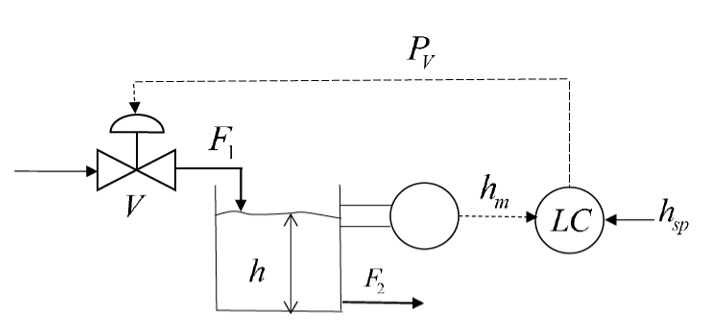
\includegraphics[width=\columnwidth]{figs/control.png}
    \caption{Process and instrumentation diagram for level control by regulating valve $V$.}
\end{figure}
\begin{enumerate}
    \item $F_1$ only
    \item $F_2$ only
    \item $h_m$ and $P_V$ only
    \item $h_{sp}$ and $P_V$ only
\end{enumerate}
\hfill (GATE BT 2021)


\item There are five bags each containing identical sets of ten distinct chocolates. One chocolate is picked from each bag. The probability that at least two chocolates are identical is

\begin{enumerate}
\item $0.3024$
\item $0.4235$
\item $0.6976$
\item $0.8125$
\end{enumerate}

\hfill (GATE BT 2021)

\item is to surgery as writer is to \\
Which one of the following options maintains a similar logical relation in the above sentence?

\begin{enumerate}
\item $Plan,\ outline$
\item $Hospital,\ library$
\item $Doctor,\ book$
\item Medicine,\ grammar
\end{enumerate}

\hfill (GATE BT 2021)

\item In adsorption chromatography, the adsorption of uncharged solute molecules onto a silica-based stationary phase is by
\begin{enumerate}
    \item covalent bonds
    \item electrostatic interactions
    \item ionic bonds
    \item van der Waals forces
\end{enumerate}
\hfill (GATE BT 2021)

\item Which one of the following statements is correct in the context of thermodynamics?
\begin{enumerate}
    \item In a closed system, neither mass nor energy is transferred across the system boundary
    \item In a closed system, both mass and energy can be transferred across the system boundary
    \item The total energy of the system is the sum of kinetic and potential energies
    \item In a closed system, only energy can be transferred across the system boundary and not mass
\end{enumerate}
\hfill (GATE BT 2021)

\item In Neurospora crassa, a mutation in the poky gene results in a slow-growth phenotype (poky). The results of four crosses are given below:
\[
\begin{aligned}
(1)\; \text{wild-type} \times \text{wild-type} &\;\rightarrow\; \text{All progeny are wild-type} \\
(2)\; \text{wild-type} \times poky &\;\rightarrow\; \text{All progeny are wild-type} \\
(3)\; poky \times \text{wild-type} &\;\rightarrow\; \text{All progeny are poky} \\
(4)\; poky \times poky &\;\rightarrow\; \text{All progeny are poky}
\end{aligned}
\]
Which one of the following explains the inheritance mode of poky?
\begin{enumerate}
    \item Episomal inheritance
    \item Mendelian inheritance
    \item Mitochondrial inheritance
    \item X-linked inheritance
\end{enumerate}
\hfill (GATE BT 2021)

\item A feed stream ($F_1$) containing components A and B is processed in a system comprising a separation unit and a mixer as shown in the schematic below. The mole fractions of components A and B are $x_A$ and $x_B$, respectively. If $F_1 + F_2 = 100\ \mathrm{kg\,h^{-1}}$, the degrees of freedom of the system is
\begin{figure}
    \centering
    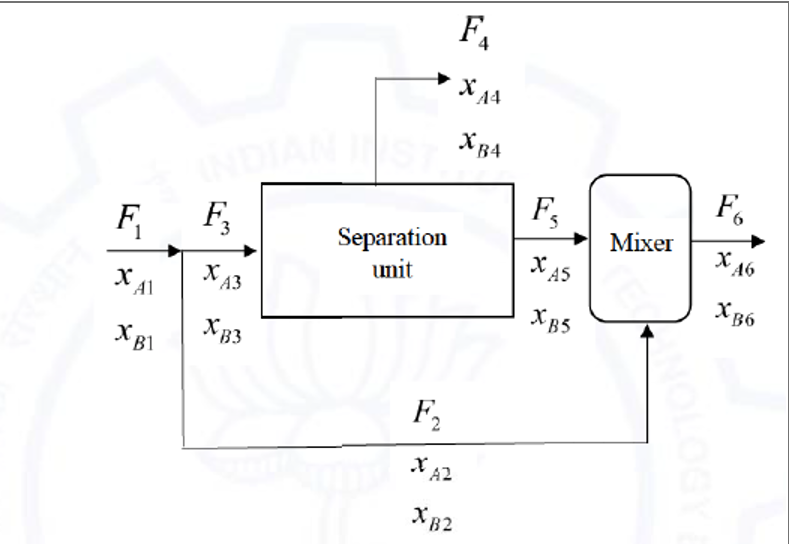
\includegraphics[width=\columnwidth]{figs/unit.png}
    \caption{Schematic of separation unit and mixer.}
\end{figure}
\hfill (GATE BT 2021)


\item Some people suggest anti-obesity measures (AOM) such as displaying calorie information in restaurant menus. Such measures sidestep addressing the core problems that cause obesity: poverty and income inequality.\\
Which one of the following statements summarizes the passage?

\begin{enumerate}
\item The proposed AOM addresses the core problems that cause obesity.
\item If obesity reduces, poverty will naturally reduce, since obesity causes poverty.
\item AOM are addressing the core problems and are likely to succeed.
\item AOM are addressing the problem superficially.
\end{enumerate}

\hfill (GATE BT 2021)
\item It is desired to scale-up a fermentation from 1 L to 1000 L vessel by maintaining a constant power-to-volume ratio. The small fermenter is operated at an agitator speed of 300 rotations per minute (rpm). If the value of scale-up factor is 10, agitator speed in rpm (rounded off to the nearest integer) for the large fermenter is
\hfill (GATE BT 2021)


\item Coronavirus genome consists of

\begin{enumerate}
\item double-stranded DNA
\item double-stranded RNA
\item negative-sense single-stranded RNA
\item positive-sense single-stranded RNA
\end{enumerate}

\hfill (GATE BT 2021)

\item The enzyme that transcribes the eukaryotic genes encoding precursor ribosomal RNAs (pre-rRNAs) of 28S, 18S and 5.8S rRNAs is

\begin{enumerate}
\item RNA polymerase I
\item RNA polymerase II
\item RNA polymerase III
\item RNA polymerase IV
\end{enumerate}

\hfill (GATE BT 2021)

\item Number of unrooted trees in a phylogeny of five sequences is

\begin{enumerate}
\item $3$
\item $15$
\item $105$
\item $945$
\end{enumerate}

\hfill (GATE BT 2021)

\item Which one of the following methods is used to test the significance of a predicted phylogeny?

\begin{enumerate}
\item Bootstrap
\item Maximum likelihood
\item Maximum parsimony
\item Minimum evolution
\end{enumerate}

\hfill (GATE BT 2021)

\item The Cartesian coordinates $(x, y)$ of a point A with polar coordinates $(4, \pi/4)$ is

\begin{enumerate}
\item $(3,2\sqrt{3})$
\item $(2, 2\sqrt{3})$
\item $(4,4\sqrt{2})$
\item $(3,4\sqrt{2})$
\end{enumerate}

\hfill (GATE BT 2021)

\item Which one of the following statements is INCORRECT about hybridoma production?

\begin{enumerate}
\item Hybridoma cells can utilise hypoxanthine and thymidine
\item DNA synthesis in myeloma cells is blocked by aminopterin
\item Hybridoma cells are made to produce polyclonal antibodies
\item Polyethylene glycol is used to fuse myeloma cells to B-cells
\end{enumerate}

\hfill (GATE BT 2021)

\item $\dfrac{d}{dx}\big[\ln(2x)\big]$ is equal to

\begin{enumerate}
\item $1/2x$
\item $1/x$
\item $1/2$
\item $x$
\end{enumerate}

\hfill (GATE BT 2021)

\item Which one of the following techniques/tools is NOT used for inserting a foreign gene into a cell?

\begin{enumerate}
\item DNA microarray
\item Electroporation
\item Gene gun
\item Microinjection
\end{enumerate}

\hfill (GATE BT 2021)

\item Under standard temperature ($T$) and pressure ($P$) conditions, $128\,g$ of an ideal gas molecule A occupies a volume of $1\,L$. The gas molecule A obeys the relationship $RT = 0.25\,PV$. $R$ and $V$ are universal gas constant and ideal gas volume, respectively. The molecule A is

\begin{enumerate}
\item CO$_2$
\item H$_2$
\item N$_2$
\item O$_2$
\end{enumerate}

\hfill (GATE BT 2021)

\item CRISPR-Cas system is associated with

\begin{enumerate}
\item adaptive immunity in eukaryotes
\item adaptive immunity in prokaryotes
\item innate immunity in eukaryotes
\item innate immunity in prokaryotes
\end{enumerate}

\hfill (GATE BT 2021)

\item The process by which intracellular macromolecules are supplied for lysosomal degradation during nutrient starvation is

\begin{enumerate}
\item apoptosis
\item autophagy
\item phagocytosis
\item pinocytosis
\end{enumerate}

\hfill (GATE BT 2021)

\item A protein without its prosthetic group is known as

\begin{enumerate}
\item apoprotein
\item hemoprotein
\item holoprotein
\item lipoprotein
\end{enumerate}

\hfill (GATE BT 2021)

\item The enzyme which adds phosphate group to the free $5'$ terminus of a DNA sequence is

\begin{enumerate}
\item adenosine kinase
\item alkaline phosphatase
\item polynucleotide kinase
\item terminal deoxynucleotidyl transferase
\end{enumerate}

\hfill (GATE BT 2021)

\item Which one of the following is CORRECT about microbial growth medium?

\begin{enumerate}
\item Luria-Bertani broth is a synthetic medium
\item Nutrient broth is a defined medium
\item Sabouraud dextrose agar is a differential medium
\item Trypticase soy agar is a complex medium
\end{enumerate}

\hfill (GATE BT 2021)

\item The cellular process which utilizes RNA-induced silencing complex to block gene expression is

\begin{enumerate}
\item RNA editing
\item RNA interference
\item RNA polyadenylation
\item RNA splicing
\end{enumerate}

\hfill (GATE BT 2021)

\item Which of the following layer(s) is/are formed from the inner cell mass of the blastocyst?

\begin{enumerate}
\item Ectoderm
\item Endoderm
\item Mesoderm
\item Trophectoderm
\end{enumerate}

\hfill (GATE BT 2021)

\item Which of the following cell organelle(s) is/are surrounded by a single phospholipid membrane?

\begin{enumerate}
\item Golgi apparatus
\item Lysosome
\item Mitochondria
\item Nucleus
\end{enumerate}

\hfill (GATE BT 2021)

\item The sum of the infinite geometric series $1 + \frac{1}{3} + \frac{1}{3^2} + \frac{1}{3^3} + \cdots$ (rounded off to one decimal place) is

\hfill (GATE BT 2021)

\item Three balls, colored in blue, green and red, are successively transferred from box A to box B in the order BLUE-GREEN-RED. The probability of a reverse transfer of the balls to the box in the same order (rounded off to two decimal places) is

\hfill (GATE BT 2021)

\item Decimal reduction time of a bacterial strain is $20$ min. Specific death rate constant in min$^{-1}$ (rounded off to two decimal places) is

\hfill (GATE BT 2021)

\item The value of $\lim_{x\to 0}\dfrac{x-\sin 2x}{x-\sin 5x}$ (rounded off to two decimal place is

\hfill (GATE BT 2021)

\item A system consists of two reactors, connected by a valve. The first reactor (A1) contains an ideal gas A of volume $5$ L and the second reactor (A2) has an ideal gas B of volume $10$ L. Initially, the valve is closed and pressure $P$ in A1 and A2 are $9$ and $6$ atm, respectively. Later, when the valve is opened, the system reaches equilibrium. If the temperature $T$ of both the reactors is maintained constant, the final equilibrium pressure in atm of the system is

\hfill (GATE BT 2021)

\item The enzyme $\alpha$-amylase used in starch hydrolysis has an affinity constant $K_p$ value of $0.005 \,\text{M}$. To achieve one-fourth of the maximum rate of hydrolysis, the required starch concentration in mM (rounded off to two decimal places) is
\begin{enumerate}
\item $1.67$
\item $2.50$
\item $3.33$
\item $5.00$
\end{enumerate}
\hfill (GATE BT 2021)

\item Match enzymes in Group I with their corresponding industrial application in Group II.\\[2pt]
Group I \hspace{3cm} Group II\\
P.\ Amylase \hspace{2.6cm} 1.\ Laundry detergent\\
Q.\ Invertase \hspace{2.5cm} 2.\ Fruit juice clarification\\
R.\ Pectinase \hspace{2.5cm} 3.\ Liquefaction of sucrose\\
S.\ Xylanase \hspace{2.55cm} 4.\ Pulp and paper processing
\begin{enumerate}
\item (A) P-2, Q-3, R-4, S-1
\item (B) P-1, Q-3, R-2, S-4
\item (C) P-1, Q-2, R-3, S-4
\item (D) P-1, Q-4, R-2, S-3
\end{enumerate}
\hfill (GATE BT 2021)

\item Match separation methods in Group I with associated properties in Group II.\\[2pt]
Group I \hspace{3.5cm} Group II\\
P.\ Centrifugation \hspace{2.2cm} 1.\ Density\\
Q.\ Dialysis \hspace{3.5cm} 2.\ Diffusivity\\
R.\ Solvent extraction \hspace{1.8cm} 3.\ Size\\
S.\ Ultrafiltration \hspace{2.7cm} 4.\ Solubility
\begin{enumerate}
\item (A) P-4, Q-2, R-1, S-3
\item (B) P-3, Q-1, R-2, S-4
\item (C) P-1, Q-3, R-2, S-4
\item (D) P-1, Q-2, R-4, S-3
\end{enumerate}
\hfill (GATE BT 2021)

\item Match the autoimmune diseases in Group I with the corresponding primarily affected organ in Group II.\\[2pt]
Group I \hspace{3.5cm} Group II\\
P.\ Hashimoto's disease \hspace{2.0cm} 1.\ Brain\\
Q.\ Juvenile diabetes \hspace{2.7cm} 2.\ Pancreas\\
R.\ Multiple sclerosis \hspace{2.6cm} 3.\ Skeletal muscle\\
S.\ Myasthenia gravis \hspace{2.7cm} 4.\ Thyroid
\begin{enumerate}
\item (A) P-1, Q-2, R-3, S-4
\item (B) P-3, Q-1, R-2, S-4
\item (C) P-4, Q-2, R-1, S-3
\item (D) P-1, Q-2, R-4, S-3
\end{enumerate}
\hfill (GATE BT 2021)

\item Match hypersensitivity types in Group I with their corresponding condition in Group II.\\[2pt]
Group I \hspace{3.5cm} Group II\\
P.\ Type I \hspace{3.7cm} 1.\ Erythroblastosis fetalis\\
Q.\ Type II \hspace{3.5cm} 2.\ Host reaction to bee venom\\
R.\ Type III \hspace{3.2cm} 3.\ Systemic lupus erythematosus\\
S.\ Type IV \hspace{3.3cm} 4.\ Tuberculin reaction
\begin{enumerate}
\item (A) P-2, Q-3, R-1, S-4
\item (B) P-3, Q-1, R-4, S-2
\item (C) P-2, Q-3, R-4, S-1
\item (D) P-2, Q-1, R-3, S-4
\end{enumerate}
\hfill (GATE BT 2021)

\item Which of the following combinations of plant hormones and their associated function are CORRECT?\\[2pt]
Hormone \hspace{3.5cm} Function\\
P.\ Abscisic acid \hspace{2.6cm} Breaks seed dormancy\\
Q.\ Auxin \hspace{3.7cm} Induces cell division\\
R.\ Ethylene \hspace{3.3cm} Stimulates ripening of fruits\\
S.\ Gibberellin \hspace{3.1cm} Promotes seed dormancy
\begin{enumerate}
\item (A) P and R only
\item (B) P and S only
\item (C) Q and R only
\item (D) Q and S only
\end{enumerate}
\hfill (GATE BT 2021)

\item Which one of the following tools is used to compare all the possible six-open reading frames of a given nucleotide query sequence with all the available six-open reading frames of the nucleotide sequence database?
\begin{enumerate}
\item (A) BLASTN
\item (B) BLASTX
\item (C) TBLASTN
\item (D) TBLASTX
\end{enumerate}
\hfill (GATE BT 2021)

\item Tertiary structure of a protein consisting of $\alpha$-helices and $\beta$-strands can be determined by
\begin{enumerate}
\item (A) Circular dichroism spectroscopy
\item (B) Mass spectrometry
\item (C) Nuclear magnetic resonance spectroscopy
\item (D) UV spectroscopy
\end{enumerate}
\hfill (GATE BT 2021)

\item Which of the following statement(s) is/are CORRECT about \textit{Agrobacterium}?
\begin{enumerate}
\item (A) It contains tumor inducing plasmid
\item (B) It causes crown gall disease in dicotyledonous plants
\item (C) It is a Gram-positive soil bacterium
\item (D) It is used in generating transgenic plants
\end{enumerate}
\hfill (GATE BT 2021)

\item Which of the following antimicrobial agent(s) is/are growth factor analog(s)?
\begin{enumerate}
\item (A) 5-Fluorouracil
\item (B) Isoniazid
\item (C) Sulfanilamide
\item (D) Tetracycline
\end{enumerate}
\hfill (GATE BT 2021)

\item Which of the following chemical messenger(s) is/are derivative(s) of tryptophan?
\begin{enumerate}
\item (A) $\gamma$-amino butyric acid
\item (B) Indole acetic acid
\item (C) Melatonin
\item (D) Serotonin
\end{enumerate}
\hfill (GATE BT 2021)

\item Which of the following nucleus/nuclei is/are NMR active?
\begin{enumerate}
\item (A) $^{1}H$
\item (B) $^{13}C$
\item (C) $^{16}O$
\item (D) $^{32}S$
\end{enumerate}
\hfill (GATE BT 2021)

\item In a Mendel's dihybrid experiment, a homozygous pea plant with round yellow seeds was crossed with a homozygous plant with wrinkled green seeds. $F_1$ intercross produced $560$ $F_2$ progeny. The number of $F_2$ progeny having both dominant traits (round and yellow) is
\hfill (GATE BT 2021)

\item A $0.1$ mL aliquot of a bacteriophage stock having a concentration of $4\times 10^{9}$ phages mL$^{-1}$ is added to $0.5$ mL of \textit{E.\ coli} culture having a concentration of $2\times 10^{8}$ cells mL$^{-1}$. The multiplicity of infection is
\hfill (GATE BT 2021)

\item If the area of a triangle with the vertices $(k, 0)$, $(2, 0)$ and $(0, -2)$ is $2$ square units, the value of $k$ is
\hfill (GATE BT 2021)

\item In a chemostat with a dilution rate of $0.8$ h$^{-1}$, the steady state biomass concentration and the specific product formation rate are $8$ mol m$^{-3}$ and $0.2$ (mol product)(mol biomass)$^{-1}$ h$^{-1}$, respectively. The steady state product concentration in mol m$^{-3}$ is
\hfill (GATE BT 2021)

\item If the values of two random variables $(X, Y)$ are $(121, 360)$, $(242, 361)$ and $(363, 362)$, the value of the correlation coefficient between $X$ and $Y$ (rounded off to one decimal place) is
\hfill (GATE BT 2021)

\item It is desired to scale-up a fermentation from $1$ L to $1000$ L vessel by maintaining a constant power-to-volume ratio. The small fermenter is operated at an agitator speed of $300$ rotations per minute (rpm). If the value of scale-up factor is $10$, agitator speed in rpm (rounded off to the nearest integer) for the large fermenter is
\hfill (GATE BT 2021)

\item The specific growth rate of a mold during exponential phase of its growth in a batch cultivation is $0.15$ h$^{-1}$. If the cell concentration at $30$ h is $33$ g L$^{-1}$, the cell concentration in g L$^{-1}$ (rounded off to the nearest integer) at $24$ h is
\hfill (GATE BT 2021)

\item A sedimentation tank of height $100$ cm is used in a conventional activated sludge process to separate a suspension of spherical shaped granular sludge biomass of $0.5$ mm diameter. The viscosity of the liquid is $1$ cP. The difference in density between the suspended biomass and the liquid is $0.1$ g cm$^{-3}$. If the biomass reach their terminal velocity instantaneously, the biomass settling time in min (rounded off to two decimal places) is
\hfill (GATE BT 2021)

\item In a random mating population, $Y$ and $v$ are dominant and recessive alleles, respectively. If the frequency of $Y$ allele in both sperm and egg is $0.70$, then the frequency of $Y/v$ heterozygotes (rounded off to two decimal places) is
\hfill (GATE BT 2021)

\item 
\[
\int_{0}^{\pi^2/4} \sin \sqrt{x} \, dx = \, \_\_\_\_\_ .
\]
\hfill (GATE BT 2021)

\item A batch cultivation of \textit{E.\ coli} follows zeroth-order Monod's growth kinetics. The cell growth is terminated when the residual dissolved oxygen concentration attains $10\%$ of its saturation value and oxygen mass transfer coefficient ($k_L a$) reaches its maximum value ($80\,\text{h}^{-1}$). The saturation value of dissolved oxygen concentration is $0.007\,\text{kg}\,\text{m}^{-3}$. If the maximum specific growth rate and yield coefficient ($Y_{X/O_2}$) are $0.2\,\text{h}^{-1}$ and $1.5$ (kg cells)(kg $O_2$)$^{-1}$, respectively, then the final cell concentration in $\text{kg}\,\text{m}^{-3}$ (rounded off to two decimal places) at the end of the batch cultivation is
\hfill (GATE BT 2021)

\item Milk flowing through a stainless steel inner tube ($40$ mm inner diameter) of a double tube-type heater is to be heated from $10^\circ$C to $85^\circ$C by saturated steam condensing at $120^\circ$C on the outer surface of the inner tube. Total heat transferred ($Q$) is $146200$ kcal h$^{-1}$ and the overall heat transfer coefficient is $750$ kcal h$^{-1}$ m$^{-2}$ $^\circ$C$^{-1}$. The total length of the heating tube in m (rounded off to one decimal place) is
\hfill (GATE BT 2021)

\item A DNA solution of $50\,\mu g\,mL^{-1}$ concentration gives an absorbance of $1.0$ at $260$ nm. An aliquot of $20\,\mu L$ from a $50\,\mu L$ purified plasmid solution is diluted with distilled water to a total volume of $1000\,\mu L$. The diluted plasmid solution gives an absorbance of $0.550$ at $260$ nm. The concentration of the purified plasmid in $\mu g\,\mu L^{-1}$ (rounded off to two decimal places) is
\hfill (GATE BT 2021)

\item The possible number of SalI restriction sites in a $9$ kb double-stranded DNA, with all four bases occurring in equal proportion (rounded off to the nearest integer) is
\hfill (GATE BT 2021)

\item A bacterium produces acetic acid from ethanol as per the following reaction
\[
2CH_3CH_2OH + 2O_2 \rightarrow 2CH_3COOH + 2H_2O
\]
The thermodynamic maximum yield of acetic acid from ethanol in $g\,g^{-1}$ (rounded off to two decimal places) is
\hfill (GATE BT 2021)

\end{enumerate}
\end{document}


\item Match separation methods in Group I with associated properties in Group II.\\[2pt]
Group I \hspace{3.5cm} Group II\\
P.\ Centrifugation \hspace{2.2cm} 1.\ Density\\
Q.\ Dialysis \hspace{3.5cm} 2.\ Diffusivity\\
R.\ Solvent extraction \hspace{1.8cm} 3.\ Size\\
S.\ Ultrafiltration \hspace{2.7cm} 4.\ Solubility
\begin{enumerate}
\item (A) P-4, Q-2, R-1, S-3
\item (B) P-3, Q-1, R-2, S-4
\item (C) P-1, Q-3, R-2, S-4
\item (D) P-1, Q-2, R-4, S-3
\end{enumerate}
\hfill (GATE BT 2021)

